\documentclass[11pt, a4paper]{article}
\usepackage[utf8]{inputenc}
\usepackage[T1]{fontenc}
\usepackage{helvet}
\renewcommand{\familydefault}{\sfdefault}
\usepackage[table]{xcolor}
\definecolor{schoolgreen}{HTML}{92D050}
\usepackage{geometry}
\geometry{landscape, margin=2cm, top=4cm, headheight=2.5cm, headsep=0.5cm}
\usepackage{array}
\usepackage{longtable}
\usepackage{graphicx}
\usepackage{fancyhdr}

\pagestyle{fancy}
\fancyhf{}
\fancyhead[L]{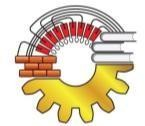
\includegraphics[height=2cm]{../../distritos/4117/templates/logo1.jpg}}
\fancyhead[R]{
\includegraphics[height=2cm]{../../distritos/4117/templates/logo2.jpg}}
\fancyhead[C]{\fontsize{10}{12}\selectfont \textbf{\textit{ESCUELA N.° 4-117 EJÉRCITO DE LOS ANDES \\ DIRECCIÓN DE EDUCACIÓN TÉCNICA Y TRABAJO \\ SECCIÓN V}}}
\renewcommand{\headrulewidth}{0pt}

\begin{document}

\noindent\colorbox{schoolgreen}{\begin{minipage}{\dimexpr\textwidth-2\fboxsep}\centering \textbf{\fontsize{14}{16}\selectfont PROGRAMA 2026}\end{minipage}}

\vspace{1em}

\begin{flushleft}
\textbf{Espacio Curricular:} Mecánica de los Fluidos \\
\textbf{Ciclo Lectivo:} 2026 \\
\textbf{Curso:} 5to 3ra \\
\textbf{Profesor/a Responsable:} Ferreyra Gustavo David
\end{flushleft}

\vspace{1em}

\begin{longtable}{|p{\dimexpr\textwidth-2\tabcolsep-2\arrayrulewidth}|}
\hline
\rowcolor{gray!20} \textbf{Contenidos Programáticos} \\
\hline
\textbf{EJE Nº 1: FUNDAMENTOS DE LA FLUIDODINÁMICA Y MECÁNICA DE FLUIDOS} \\
$\bullet$ Hidrostática: Presión, Principio de Pascal y Principio de Arquímedes. \\
$\bullet$ Hidrodinámica: Ecuaciones de continuidad, Teorema de Bernoulli y Número de Reynolds. \\
$\bullet$ Fenómenos Críticos: Cavitación, Ondas de choque y Estabilidad Hidrodinámica. \\
$\bullet$ Aplicaciones Técnicas: Simbología de fluidos, Cálculo de recipientes sometidos a presión y análisis de Pérdida de Carga. \\
\hline
\textbf{EJE Nº 2: INSTALACIONES Y EQUIPOS OLEOHIDRAULICOS E HIDRÁULICOS} \\
$\bullet$ Equipos y componentes hidráulicos: funciones y aplicaciones. \\
$\bullet$ Bombas hidráulicas: centrífugas y de desplazamiento positivo. \\
$\bullet$ Ensayos de bombas y rendimiento. \\
$\bullet$ Circuitos de comando de instalaciones y máquinas. \\
$\bullet$ Turbinas: Pelton, Francis, Kaplan y Bulbo. \\
$\bullet$ Bombas radiales, axiales, mixtas y de vacío. \\
$\bullet$ Frenos hidráulicos. \\
$\bullet$ Sistemas oleohidráulicos: componentes básicos y lógica de funcionamiento. \\
$\bullet$ Esquematización de circuitos oleohidráulicos. \\
$\bullet$ Equipos oleohidráulicos: prensas, carga, transporte, elevación y compactación. \\
$\bullet$ Presiones admisibles y medidas de seguridad. \\
\hline
\textbf{EJE Nº 3: INSTALACIONES Y EQUIPOS NEUMÁTICOS} \\
$\bullet$ Componentes de sistemas neumáticos y principios teóricos. \\
$\bullet$ Dimensionado de tuberías para transporte de caudales. \\
$\bullet$ Parámetros funcionales: presiones, velocidades, caudales. \\
$\bullet$ Ecuaciones de fluidodinámica aplicables a los gases. \\
$\bullet$ Sistemas de producción y utilización. \\
$\bullet$ Componentes de producción: compresores, presostatos, cilindros, válvulas de seguridad, filtros, trampas de agua y lubricación. \\
$\bullet$ Cálculo de capacidad en cilindros y protección ante humedad. \\
$\bullet$ Componentes electroneumáticos y automatización. \\
$\bullet$ Ventiladores, soplantes y extractores. \\
$\bullet$ Automatización de sistemas neumáticos: componentes, fuerzas y tiempos de accionamiento. \\
$\bullet$ Componentes de utilización: válvulas, actuadores y lógica de circuitos. \\
\hline
\textbf{EJE Nº 4: ELEMENTOS DE MEDICIÓN Y ENSAYOS} \\
$\bullet$ Caracterización de tipos de ensayos referidos a fluidos. \\
$\bullet$ Pruebas de estanqueidad y pruebas hidráulicas según normas. \\
$\bullet$ Mediciones de caudal y presión en cañerías y depósitos. \\
$\bullet$ Variables en el cálculo y diseño de instalaciones hidráulicas. \\
$\bullet$ Instrumentos de medición: caudalímetro, manómetro relativo y absoluto, piezómetro. \\
\hline
\end{longtable}

\end{document}